\section{Task Analysis}
\label{sec:task}
%Identifying the analysis goals and the corresponding visualization tasks is the first significant step in designing a useful tool. 
%In this section, we examine how domain experts normally approach the task of analyzing a model (i.e., assess its strength and weakness) and identify where and how an interactive visualization system can aid in such a process.
%\shusen{
The primary driving force for designing the proposed tool is the error analysis challenges faced by our long-term collaborators working on natural language inference research. During the entire design and development process, we worked closely with two NLP experts via weekly meetings in a period of roughly seven month, their constant evaluation and feedback have helped shape the tool we see today.
%}
%Then, we distill the numerous discussions with domain experts into concrete tasks, which guide the design and implementation of the proposed tool.
%During our long-term collaboration with two NLP experts, 
During this period, we have conducted extensive discussions to understand the common approaches employed by researchers for assessing the behavior of a model.
% as well as provide feedback on the various prototyping stages of the proposed visualization.%
The predictive accuracy has its place as an objective evaluation metric to measure the overall effectiveness of the model; however, the accuracy number alone does not provide the full story.
For example, the model may produce correct predictions for the ``wrong'' reasons (e.g., pick up an unintended pattern in the training data that cannot be generalized in real-word scenarios).
%
As a result, the domain experts rely on an exploration-centric approach to conduct error analysis and obtain intuition.
%
There is little one can learn when everything is behaving as expected, and therefore,
observing how models make mistakes under various scenarios is at the center of such a process.
The experts often start with simple failure examples, and then make minor perturbations (replace a word or phrase) to the input and observe the change in the prediction. This exercise helps isolate where in the input likely contribute to the failures. For many NLP models, the attention information (see Section~\ref{sec:attention}) is essential to infer the mechanism of the model. Experts often print out the attention values or generate plots to visualize sentence alignment or compare attention values. As the experts explore more variation of similar examples, combined with their domain knowledge, they may develop hypotheses about the cause of failures, or ask additional questions that lead to further experimentation.

In such an exploration workflow, NLP researchers often need to utilize multiple scripts and manually run all the experiments. The batch process based approach, is not only time consuming, but also hinders the flow of reasoning which rely on obtaining instantaneous feedbacks, and making many on-the-fly adjustments.
%
Therefore, the expert driven exploration process can greatly benefit from the introduction of an interactive visual exploration environment, where the researchers can easily express their hypotheses and obtain quick visual feedback of the results.
%
Moreover, by introducing new visual encodings and summarizations, we can drastically expand the ways domain experts interact with the model, enable exploration options that previously were not possible either due to tedious manual operation or the lack of communication channels.
%
%In such a highly exploratory process, the expert likely will have many ``what if'' type of questions (e.g., what if I make change to this word in the input, what if I force the words to align correctly in the attention), get responsive answers to these queries is essential to maintain the flow of reasoning.
%\shusen{
To support the exploratory workflow for analyzing NLI models,
we aim to address the following tasks based on our extensive discussions with NLP experts.
%}

\begin{itemize}
    \item \textbf{T1}: Understand the stability of a prediction, i.e., how perturbations of the input affect the behavior of the model?

    \item \textbf{T2}: Examine the attention mechanism, i.e., what is the relationship between the input and the attention, and how does the attention affect the prediction?

    \item \textbf{T3}: When the predicted label is wrong, how can we update the model to correct the prediction? What are the effects of updating different parts of the model?
\end{itemize}

In Section~\ref{sec:caseStudy}, we will discussion in detail how we can utilize the proposed tool to address these tasks (the application scenarios 1,2,3 corresponds to \textbf{T1-T3}, respectively).


%\item To begin with, understanding how perturbation (e.g., replacing words with synonymous) of the input affects the prediction is the crucial part of error analysis. It not only measures the prediction sensitivity, but also helps reveal the potential source of the errors in the input (\textbf{T1}).

%Understand how attention affect the prediction.
%\item In addition, we study the role and mechanism of attention by examining how perturbation in the input sentence affect the attention, and how changes in attention affect prediction (\textbf{T2}).
%Study the relationship between model stages (encoder, attention, classifier) and the prediction

%\item So far, we focus on how changes in earlier stage of the model affect later stages or the final prediction. However, what if the current prediction is wrong, how can we apply minimal update to the model to produce correct prediction. and how would such a modification affect attention (\textbf{T3}).
% Therefore, thirdly, we want to explore how model should be updated to produce the desirable change of prediction, and how the attention respond to such a change (\textbf{T3}).

%Through many rounds of discussions with NLP experts,
%In such a highly exploratory process, the expert likely will have many ``what if'' type of questions (e.g., what if I make change to this word in the input, what if I force the words to align correctly in the attention), get responsive answers to these queries is essential to maintain the flow of reasoning.

%To support the analysis goal and visual exploratory workflow, we have summarized the following visualization tasks.

% \begin{itemize}
% \item To start with, we need to construct the visual language for communicating the model information to the user, which mean designing visual encoding for key model information, such as attention, the prediction results, as well as input sentences (T1). %but also the user interface to convey various perturbation operation (T2);
%
% \item  In addition, convey the user intend to the underlying computation is the other part of the puzzle.
% The user should be able to easily express operations such as perturb input sentences, update attention values, as well as re-assign prediction.
% % the   the role and mechanism of attention by examine how perturbation in the input sentence affect the attention, and how changes in attention affect prediction (\textbf{T2}).
%
% \item Finally, to identify the where and how the model change to  update  res we have focused on how changes in earlier stage of the model affect later stages or the final prediction. However, what if the current prediction is wrong, where and how can we apply update to the model to produce correct prediction and how the attention respond to such a change (\textbf{T3}).
%
% \end{itemize}
%
% Based on the NLP analysis goals, we identify the visualization tasks to achieve these goals.

% \begin{itemize}
% \item \textbf{T1} Visualize the \emph{input}, \emph{attention}, \emph{prediction} of the model.
% \item \textbf{T2} Automate the perturbation of the input, explore the perturbation result.
% \item \textbf{T3} Customize the \emph{attention} for studying the relationship between attention and prediction
% \item \textbf{T4} Visualize the changes in the model stages with respect to prediction change driven model update %\shusen{does not make sense}
% \end{itemize}


%interrupted when they can not easily receive the answers to their immediate queries.

% examining examples (e.g, what are the mistakes made by the model), and conduct experiments (e.g., perturb the input and observe the changes), formulate hypothesis (e.g, what are the potential causes for the failure).
%ultimate forms intuition about the strength or the weakness of a given model.
% , then additional examples or variation of existing examples are bring in to rejected or confirm the hypotheses. And new questions or hypothesis may arise.
%Such an analysis is iterative in nature and guided by domain knowledge and hypotheses based on the architecture. As they ask more questions and experiment
%experiment with model iterate their understanding of the model behavior, ultimate forms intuition about the strength or the weakness of a given model.
%and come up hypothesis about the potential cause for the failure.



%\begin{figure}[htbp]
%\centering
%\vspace{-2mm}
% 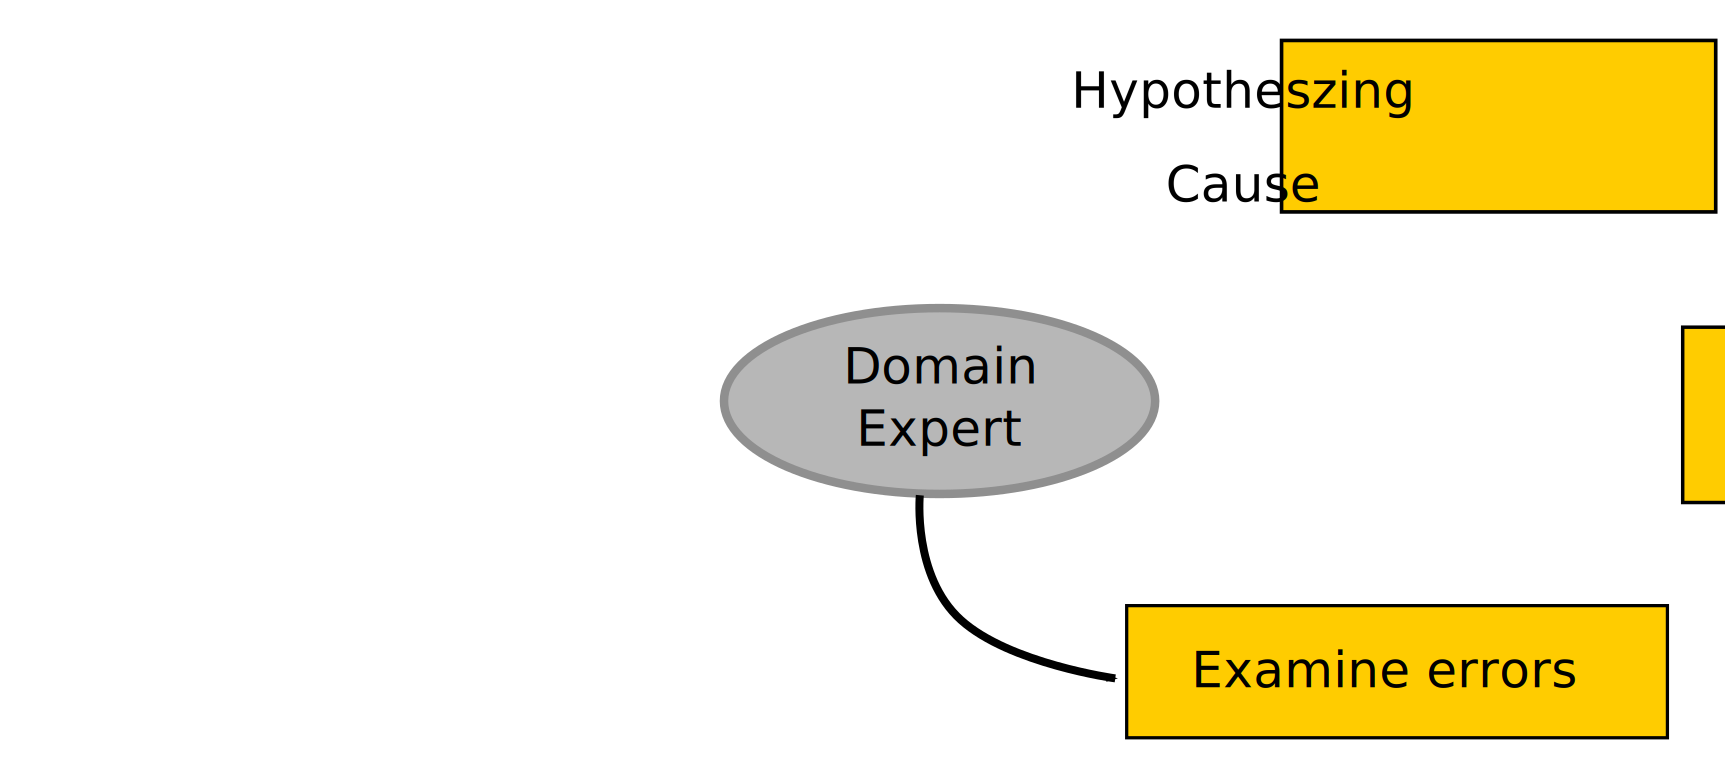
\includegraphics[width=1.0\linewidth]{errorAnalysis}
% \caption{How domain experts conduct error analysis on the model.}
%\label{fig:modelPipeline}
%\end{figure}
